\documentclass[10pt,t]{beamer}
\setbeamersize{text margin left=10pt,text margin right=10pt}
\usepackage{fancyvrb}

\usefonttheme{professionalfonts}
\usefonttheme{serif}
% Delete this, if you do not want the table of contents to pop up at
% the beginning of each subsection:
\AtBeginSection[]
{
  \begingroup
  \setbeamertemplate{background canvas}[vertical shading][bottom=lubrown,top=lubrown]
  \setbeamertemplate{footline}[myfootline] 
  \setbeamertemplate{section page}[mysection]
  \frame[c]{
    \sectionpage
  }
  \endgroup
}

\title{Constraining Cosmological and Astrophysical Parameters Using UV Luminosity Functions at z~6}
\subtitle{A Computational Approach}
\author{Aaron Kebede and Sultan Hassan}
\institute{\href{https://lehigh.edu/agk223}{Lehigh University / Flatiron CCA}}
\date{\today}

% footer logo
\pgfdeclareimage[width=0.3\paperwidth]{university-logo}{lulogo}
\tllogo{\pgfuseimage{university-logo}}

%titlepage logo
\titlegraphic{
\includegraphics[scale=0.5]{lu}}
\begin{document}

\begin{frame}
  \titlepage
\end{frame}

\begin{frame}[c]
\begin{figure}
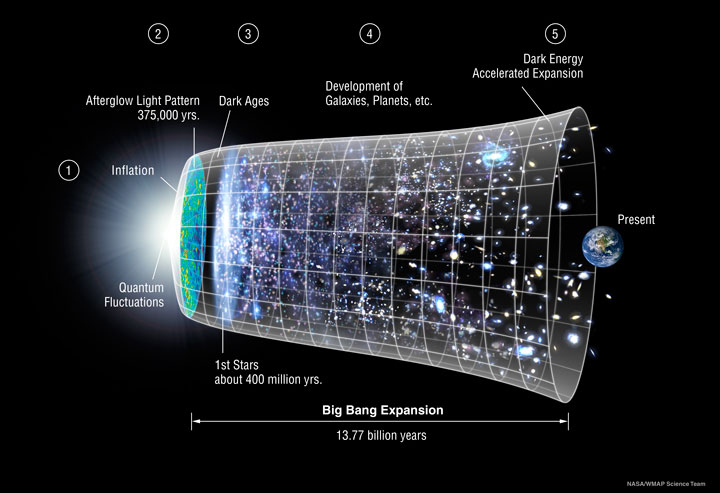
\includegraphics[width=200]{images/lambda.jpg}
\caption{The $\lambda$CDM model /Credit \textit{: NASA WMAP Team} }
  \label{fig: lambda CDM model}
\end{figure}
  \begin{itemize}
    \item Cosmology is the study of the origin and fate of the universe.
    \item The CMB is our primary source of cosmological data.
    \item The current most accepted form of cosmology is the $\lambda$CDM model which asserts the beginning of the universe with a big bang
  \end{itemize}
\end{frame}

\begin{frame}{The Standard Model }
\begin{itemize} \newline \newline
\item Makes use of a model with dark matter with non-relativistic velocities(hence, cold)
\item Can be accurately described by 6 parameters(two of which, the $\Omega_m$ and $\sigma_8$, we will attempt to constrain)
\item Most of the information about the parameters can be exctracted from the CMB data. Missions such as the WMAP and Planck collect light from the CMB.
\item By combining the parameters we can come up with a cosmological model that can tell us about the universe(e.g. expansion, age, curvature, composition & \textit{fate})
\item However, the model has its own shortcomings. For one, we are still not sure about what dark matter & gravity. And baryonic interactions are not well understood yet, which makes it difficult for simulations. 
\end{itemize}
\end{frame}
\begin{frame}{Understanding Simulations}
Simulations are of great importance in studying cosmology and astrophysics. Getting data is extremely expensive IRL and hence doing simulations helps at least in leading to the correct direction in research. \newline \newline
\begin{itemize}
    \item We use different kinds of simulations in studying cosmology. One is MHD simulations and the other is N-Body.
    \item  N-body simulations take into account the effects of gravity & hence we use them to study galaxy halos and dark matter while MHD simulations make use of fluid dynamics.
\end{itemize}
Simulations are definitely less expensive than actual probes like WMAP, but computation is extremely expensive and takes a lot of time. That is why we will be using machine learning along with the simulation data to achieve our goals( whether it is generating models or parameter estimation.
\newline \newline
\end{frame}
\begin{frame}{CAMELS(Cosmology and Astrophysics with MachinE Learning Simulations)}
CAMELS is a suite of more than 4000 N-body and MHD simulations designed for use in machine learning.
\begin{itemize}
    \item Predicting quantities that we can define the universe with as functions of cosmological & astrophysical parameters.
    \item Using machine learning to extract information from the simulation & make predictions about the observations
    \item Find mapping between different types of simulations
\end{itemize}
\begin{figure}

\includegraphics[width=90]{img/camels.png}

\includegraphics[width=90]{img/simba.png}    
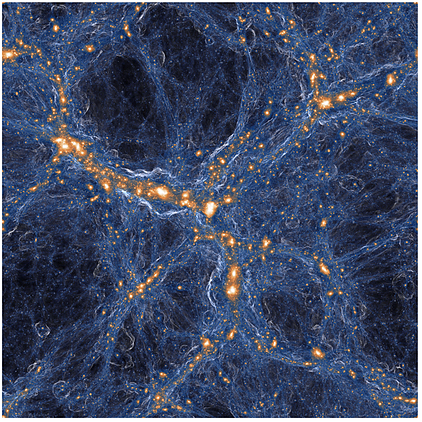
\includegraphics[width=90]{img/tng.png}    
\caption{Credit\textit{: Villaescusa-Navarro et al., and the SIMBA & TNG teams} }
  \label{fig: lambda CDM model}
\end{figure}
\end{frame}
\begin{frame}{Luminosity Functions}
\newline
\begin{figure}
    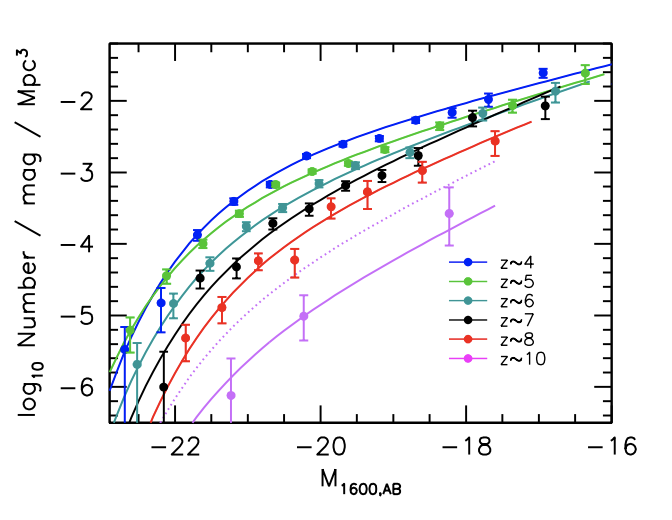
\includegraphics[width=150]{img/lfs.png}
    \caption{Bouwens et al 2015}
    
\includegraphics[width=90]{img/schechter.png}
    \caption{Schechter et al 1976}
    \label{fig:LF}
\end{figure}
Luminosity functions are distribution functions that are a measure of distribution of luminosities of objects in a sample. 
\end{frame}
\begin{frame}{Cont..}
Since it's hard to measure luminosity, we usually express LFs in terms of specific luminosity from which we can derive the magnitude. 
\newline \newline
Let's get to work. \newline \newline
Inside each suite of a simulation in CAMELS, there are different folders.
\begin{itemize}
    \item\textbf{1P}(one parameter at a time) 
    \item\textbf{CV}(cosmic variance - differ in initial random seed)
    \item\textbf{EX}(extreme-same cosmology, but different astrophysical parameters)
    \item\textbf{LH}(different parameters arranged in a latin-hypercube) folders.
\end{itemize}
\end{frame}
\end{document}